\chapter{Efficient online k-mer counting using a probabilistic data structure}


\section{Introduction}

Our motivation for exploring efficient k-mer counting comes from our
work with metagenomic data, where we routinely encounter data sets
that contain $300 \times 10^9$ bases of DNA and over 50 billion
distinct k-mers \cite{Howe2012}. 
K-mer counting plays a key role in our initial investigation on using distinct 
k-mers to measure microbial diversity. We needed to count how many distinct 
k-mers in different metagenomics data sets and get the abundance distribution. 
In the beginning we used an existing k-mer counting tool - Tallymer \cite{Kurtz2008}
. However as we started to deal with 
larger metagenomic data, where we routinely encounter data sets that contain 
300 -109 bases of DNA and over 50 billion distinct k-mers \cite{Howe2012},
it was not efficient enough and for some data set it can not handle at all. 
 Also, to efficiently filter, partition,
and assemble these data, we need to store counts for each of these
k-mers in main memory, and query and update them in realtime --- a set
of functionality not readily offered by current packages.  Moreover,
we wish to enable the use of cloud and desktop computers, which may
have poor I/O performance or limited memory. These needs have dictated
our exploration of efficient in-memory k-mer counting techniques.

In this chapter we present the khmer
software package for fast and memory efficient {\em online} counting
of k-mers in sequencing data sets. Unlike previous methods based on
data structures such as hash tables, suffix arrays, and trie
structures, khmer relies entirely on a simple probabilistic data
structure, a Count-Min Sketch.  The Count-Min Sketch permits online
updating and retrieval of k-mer counts in memory which is necessary to
support online k-mer analysis algorithms.  On sparse data sets this
data structure is considerably more memory efficient than any exact
data structure.  In exchange, the use of a Count-Min Sketch introduces
a systematic overcount for k-mers; moreover, only the counts, and not
the k-mers, are stored.

% @CTB cloud in discusson at end
We use the Amazon cloud to compare time, memory, and disk usage of our
k-mer counting implementation with that of other k-mer counting software packages, 
for two problems. First, we generate a k-mer abundance
distribution for large data sets; and second, we query many individual
k-mer counts at random from a previously constructed k-mer count
database.  We show that khmer is competitive in speed, memory, and
disk usage for these problems.  We also analyze the effects of
counting error on calculations of the k-mer count in sequencing data
sets, and in particular on metagenomic data sets. 


\section{Count-Min Sketch and its application in k-mer counting}

Below, we describe an implementation of a simple probabilistic data
structure for k-mer counting. This data structure is based on a
Count-Min Sketch \cite{Cormode2005}, a generalized probabilistic data structure for
storing the frequency distributions of distinct elements. 

Probabilistic approaches can be particularly memory efficient for
certain problems, with memory usage significantly lower than any exact
data structure \cite{Pell2012}.  However, their use introduces set
membership or counting false positives, which have effects that must
be analyzed in the context of specific problems.  Moreover, unlike
existing techniques, the Count-Min Sketch stores only counts; k-mers
must be retrieved from the original data set.  In exchange, the low
memory footprint enabled by this probabilistic approach enables online
updating and retrieval of k-mer counts entirely in memory, which in
turn supports streaming applications such as digital normalization, which will
be discussed in next chapter.

Because of the 
probabilistic characteristics of this approach, We will also discuss
the choice of optimal parameters to balance the efficiency and accuracy of k-mer 
counting.



\subsection{Implementing a Count-Min Sketch for k-mers}

The two basic operations supported by khmer are {\tt
  increment\_count(kmer) } and {\tt c = get\_count(kmer). } Both
operate on the data structure in memory, such that neither
incrementing a count nor retrieving a count involves disk access.

The implementation details are similar to those of the Bloom filter in
\cite{Pell2012}, but with the use of 8 bit counters instead of 1 bit
counters.  Briefly, Z hash tables are allocated, each with a different
size of approximately H bytes ($H_1, H_2, ..., H_Z$); the sum of these
hash table sizes must fit within available main memory.  To increment
the count for a particular k-mer, a single hash is computed for the
k-mer, and the modulus of that hash with each hash table's size H
gives the location for each hash table; the associated count in each
hash table is then incremented by 1.  We use different sizes for each
hash table so as to vary the hash function.  Even if two k-mers have
the same modulus in one hash table (a collision), they are unlikely to
collide in the other hash tables.  To retrieve the count for a k-mer,
the same hash is computed and the minimum count across all hash tables
is computed. While different in implementation detail from the
standard Bloom filter, which uses a single hash table with many
hash functions, the performance details are identical \cite{Pell2012}.
% 
One particularly important feature of the Count-Min Sketch is that the
counting error is {\em one-sided} \cite{Cormode2005}.  Because counts
are only incremented, collisions result in inflated miscounts; if
there is no collision for a particular k-mer, the count is correct.

An additional benefit of the Count-Min Sketch is that it is extremely
easy to implement correctly, needing only about 3 dozen lines of C++
code for a simple threadsafe implementation.  (We have
described how khmer scales with multiple threads in
\cite{McDonald2013}.)

To determine the expected false positive rate --- the average frequency with
which a given k-mer count will be incorrect when retrieved --- we can
look at the hash table load. Suppose N distinct k-mers have been counted
using Z hash tables, each with size H.  The probability that no
collisions happened in a specific entry in one hash table is
$(1-1/H)^{N}$, or approximately $e^{-N/H}$. The individual collision
rate in one hash table is then $\approx 1-e^{-N/H}$. The total
collision rate, which is the probability that a collision occurred in
each entry where a k-mer maps across all Z hash tables, is $\approx
(1-e^{-N/H})^{Z}$, which is also the expected false positive rate.

While the false positive rate can easily be calculated from the hash table
load, the average {\em miscount} --- the degree to which the measured
count differs from the true count --- depends on the k-mer frequency
distribution, which must be determined empirically.  We analyze the
effects of this below.


\subsection{Choosing number and size of hash tables used for k-mer counting}

The false positive rate depends on the number of distinct k-mers $N$,
the number of hash tables $Z$, and the size of the hash tables $H$: $f
\approx (1-e^{-N/H})^{Z}$, with an associated memory usage of $M = H
Z$.  We face two common scenarios: one in which we have a fixed number
of k-mers $N$ and fixed memory $M$ and we want to calculate the
optimal number of hash tables $Z$; and one in which we have a desired
maximum false positive rate $f$ and a fixed number of k-mers $N$, and
we want to calculate the minimum memory usage required to achieve $f$.

For fixed memory $M$ and number of distinct k-mers $N$, the optimal
number of hash tables can be found by minimizing $f$; taking the
derivative, $df/dZ$, with $f \approx \exp(Z \log(1-e^{-ZN/M}))$ and solving
for 0, we find that $f$ is minimized when $Z=\log(2)*(M/N)$ (see
\cite{broder2004network} for details).

Given a desired false positive rate $f$ and a fixed number of k-mers
$N$, the optimal memory usage can be calculated as follows.  First,
the optimal number of hash tables is determined by the expected false
positive rate alone: $Z = \log_{0.5}f$.  Using this $Z$, the minimum
average hash table size $H$ necessary to achieve $f$ can be calculated
as $H = (\log_{0.6185}(f)\times N)/Z$ (see
\cite{broder2004network} for details).

A remaining problem is that the number of distinct k-mers $N$ is
typically not known.  However, memory- and time-efficient algorithms
for calculating $N$ do exist and we has implemented this in
khmer\cite{flajolet2008hyperloglog}.


\section{khmer can count k-mers efficiently}


\subsection{khmer is a generally useful k-mer counting approach}


\begin{table}[!ht]
\caption{
\bf{Benchmark soil metagenome data sets for k-mer counting performance, taken from
\cite{Howe2012}.}}
\begin{tabular}{ |c | c |c| c|c| }
\hline
Data set & size of file (GB) & number of reads & number of distinct
k-mers & total number of k-mers \\
\hline
subset 1        & 1.90 &  9,744,399 &   561,178,082 &   630,207,985 \\
subset 2        & 2.17 & 19,488,798 & 1,060,354,144 & 1,259,079,821 \\
subset 3        & 3.14 & 29,233,197 & 1,445,923,389 & 1,771,614,378 \\
subset 4        & 4.05 & 38,977,596 & 1,770,589,216 & 2,227,756,662 \\
entire data set & 5.00 & 48,721,995 & 2,121,474,237 & 2,743,130,683 \\
\end{tabular}
\begin{flushleft}
\end{flushleft}
\label{table:datasets}
\end{table}


% @CTB explain why different runs
\begin{figure}[!ht]
\centerline{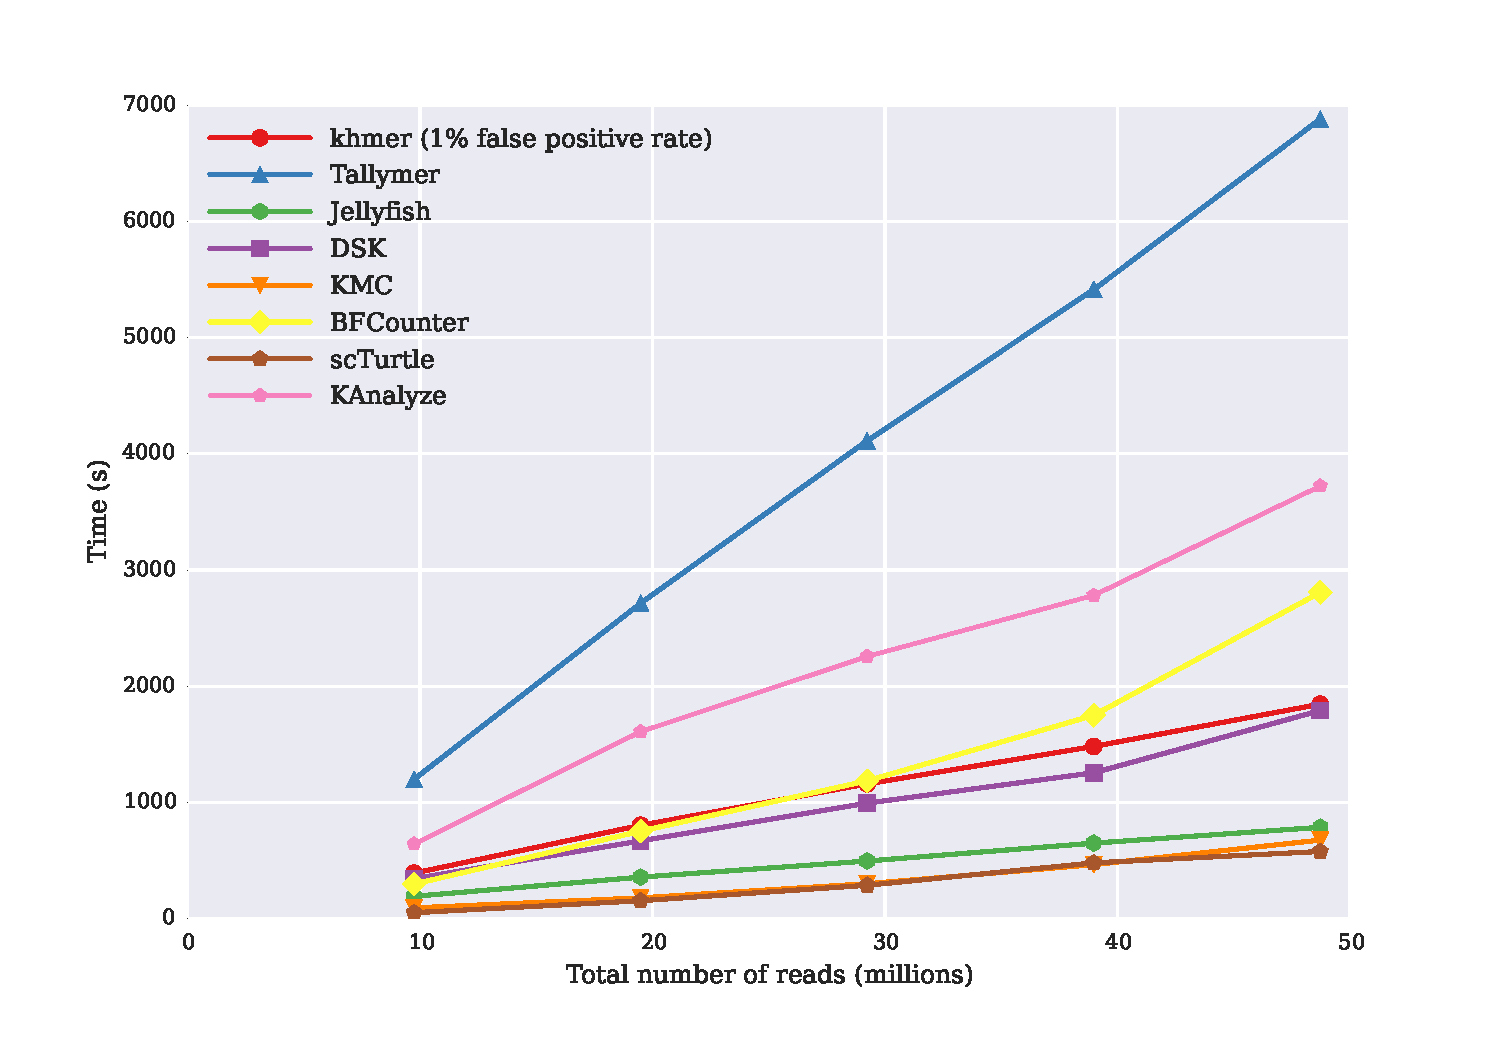
\includegraphics[width=5in]{./figures/figure1_time_benchmark}}

\caption{\bf Comparison of the time it takes for k-mer counting tools
  to calculate k-mer abundance histograms, with time (y axis, in
  seconds) against data set size (in number of reads, x axis).  
  All programs executed in time approximately linear with
  the number of input reads.}

\label{fig:cmp_time}
\end{figure}

\begin{figure}[!ht]
\centerline{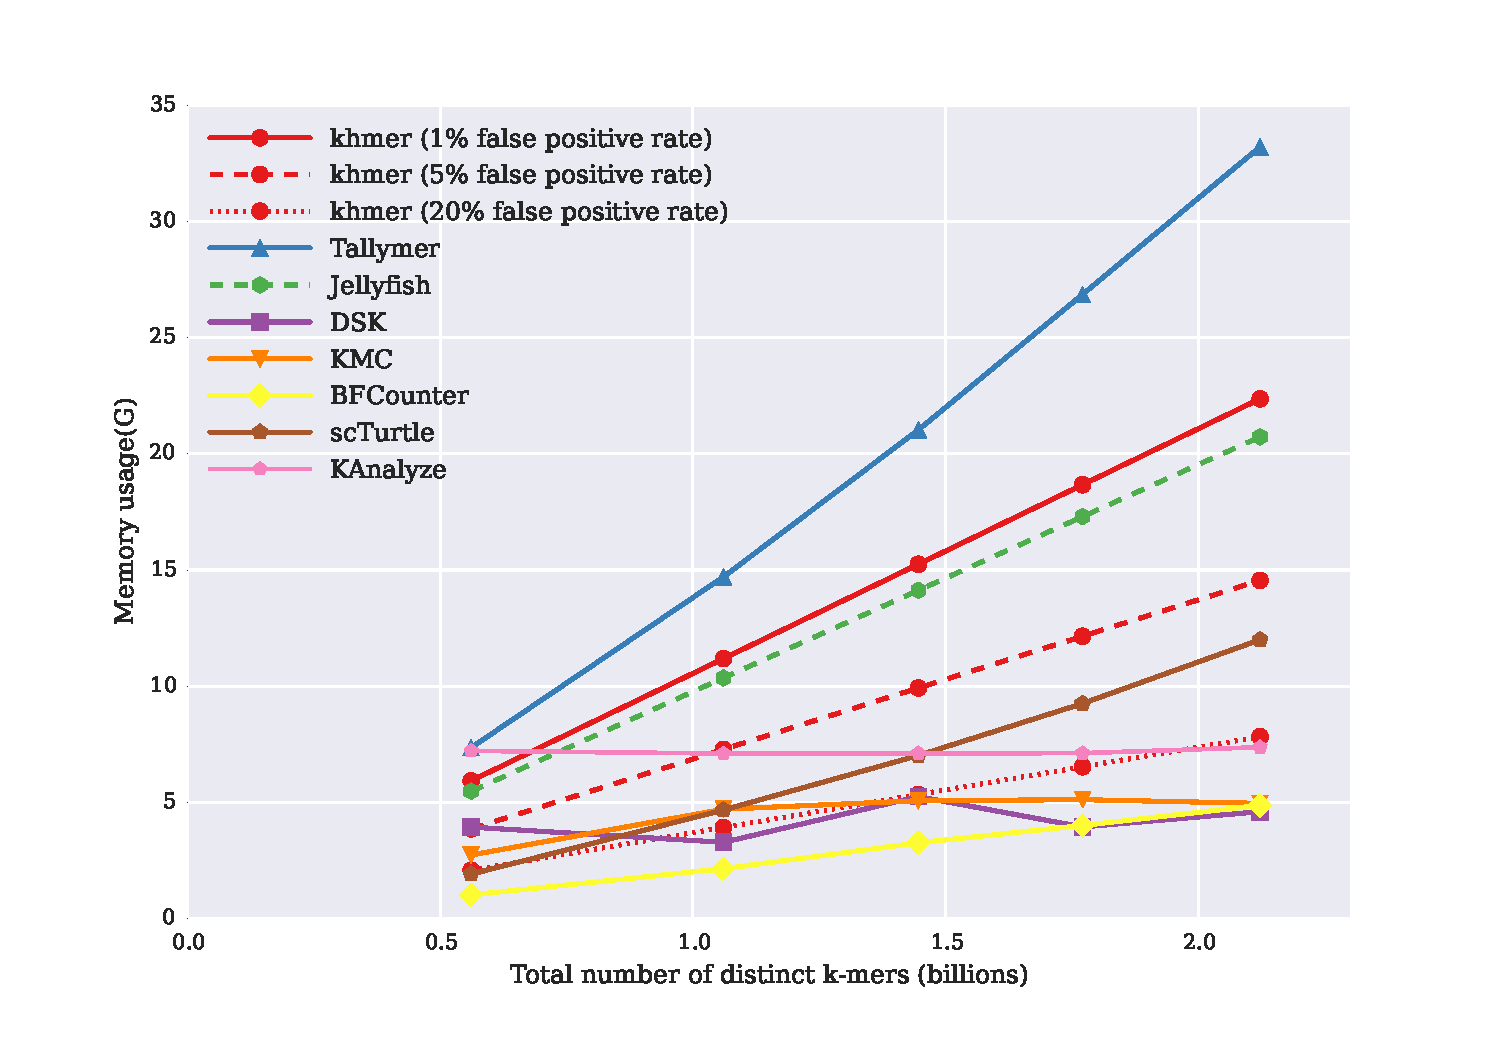
\includegraphics[width=5in]{./figures/figure2_memory_benchmark}}

\caption{\bf Memory usage of k-mer counting tools when calculating
  k-mer abundance histograms, with maximum resident program size (y
  axis, in GB) plotted against the total number of distinct k-mers in
  the data set (x axis, billions of k-mers). }

\label{fig:cmp_memory}
\end{figure}

\begin{figure}[!ht]
\centerline{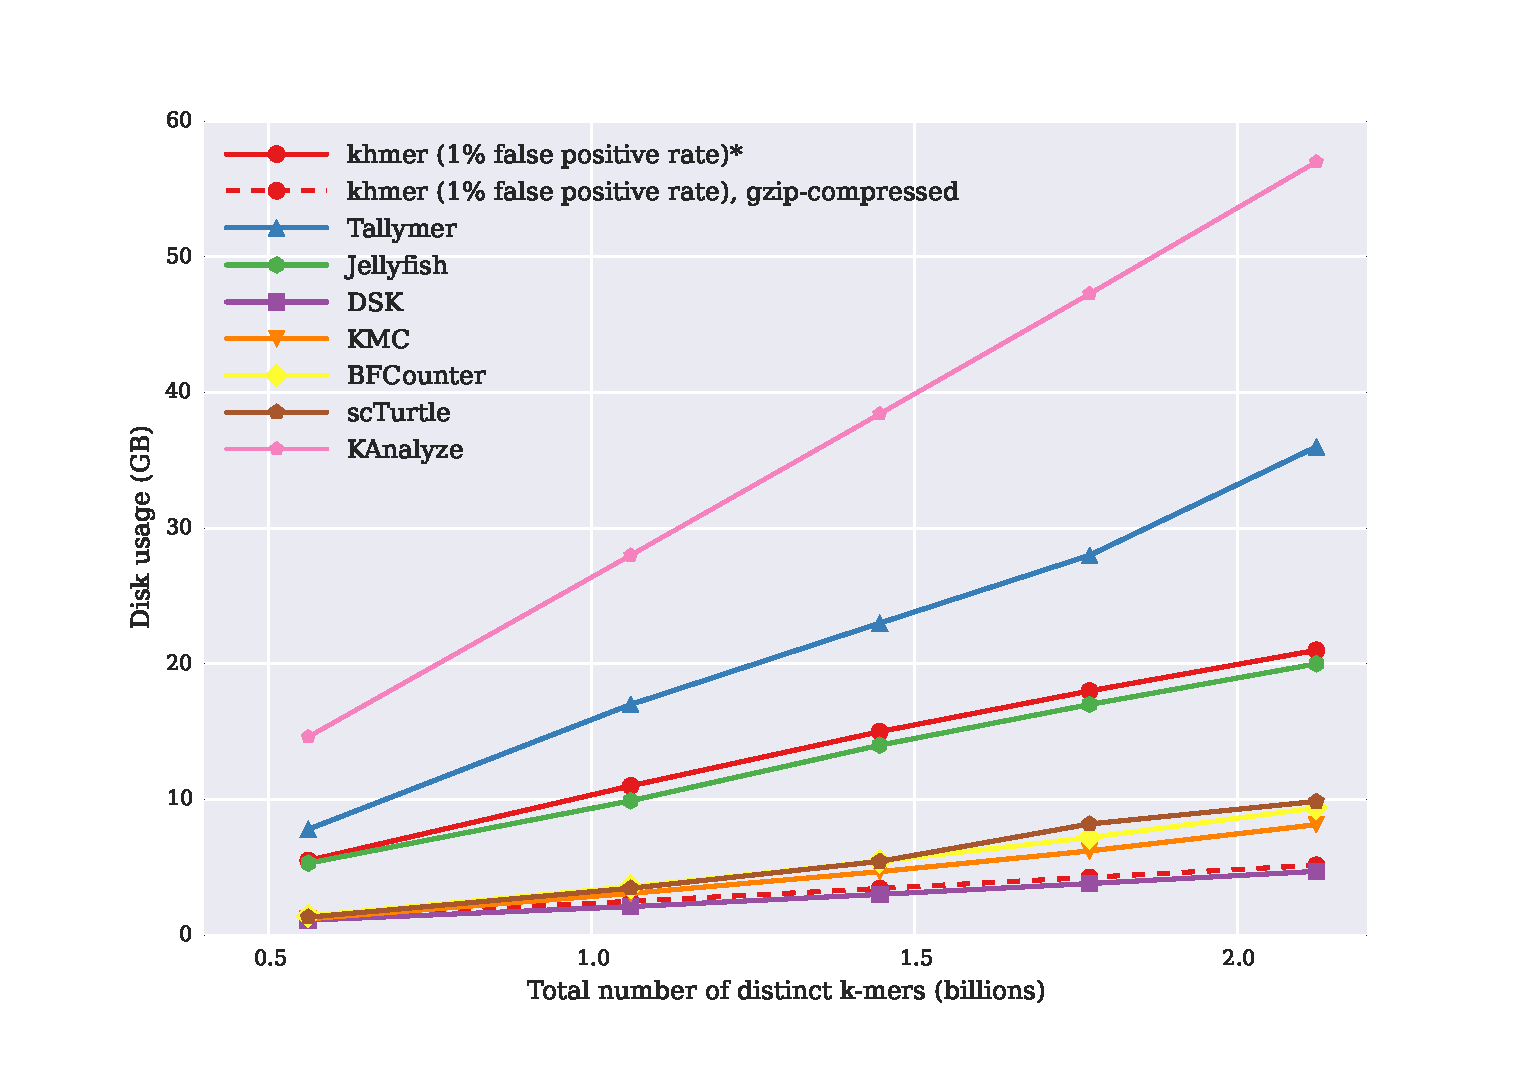
\includegraphics[width=5in]{./figures/figure3_disk_benchmark}}

\caption{\bf Disk storage usage of different k-mer counting tools to
  calculate k-mer abundance histograms in GB (y axis), plotted against
  the number of distinct k-mers in the data set (x axis).  $^*$Note
  that khmer does not use the disk during counting or retrieval,
  although its hash tables can be saved for reuse.}

\label{fig:cmp_disk}
\end{figure}

We measured time and memory required to calculate k-mer abundance
histograms in five soil metagenomic read data sets using khmer,
Tallymer, Jellyfish, DSK, KMC, Turtle, and KAnalyze (Table
\ref{table:datasets}; Figures \ref{fig:cmp_time} and
\ref{fig:cmp_memory}).  We chose to benchmark abundance histograms
because this functionality is common to all the software packages, and
is a common analysis approach for determining assembly parameters
\cite{Chikhi:2014aa}.  We applied each package to increasingly large
subsets of a 50m read soil metagenome data set \cite{Howe2012}. For
the BFCounter, KMC, Turtle and KAnalyze packages, which do not
generate k-mer abundance distribution directly, we output the
frequency of each k-mer to a file but do no further analysis.


khmer offers a general range of useful
performance tradeoffs for disk I/O, time and memory.  From the
performance comparison between khmer and other k-mer counting packages
in calculating k-mer abundance distributions, khmer is comparable with
existing packages. Figure \ref{fig:cmp_time} shows that the time usage of the khmer
approach is comparable to DSK and BFCounter, and, as expected,
increases linearly with data set size. Tallymer is the slowest of the
four tools in this testing, while KMC, Turtle, and Jellyfish are
the fastest. 
From Figure \ref{fig:cmp_memory}, we see that the memory usage of
Jellyfish, Tallymer, BFCounter, and Turtle increases linearly with
data set size. Tallymer uses more memory than Jellyfish generally,
while BFCounter and Turtle have considerably lower memory usage.
DSK, KMC, and KAnalyze use constant memory across the data sets, but
at the cost of more limited functionality (discussed below).

We also measured disk usage during counting.  Figure
\ref{fig:cmp_disk} shows that the disk usage also increases linearly
with the number of k-mers in the data set.  For a high-diversity
metagenomic data set of 5 GB, the disk usage of both Jellyfish and
Tallymer is around 30 GB.  khmer counts k-mers entirely in working
memory and does not rely on any on-disk storage to store or retrieve
k-mer counts, although for practicality the hash tables can be saved
for later reuse; the uncompressed disk usage for khmer in Figure
\ref{fig:cmp_disk} is the same as its memory.  At the expense of more
time, khmer supports saving and loading gzip-compressed hash tables,
which are competitive in size to DSK's on-disk database (Figure 3,
dashed line).


\subsection{khmer memory usage is fixed and low}

The memory usage of the basic Count-Min Sketch approach is fixed:
khmer's memory usage does not increase as data is loaded. While this
means that khmer will never crash due to memory limitations, and all
operations can be performed in main memory without recourse to disk
storage, the false positive rate may grow too high.  Therefore the
memory size must be chosen in light of the false positive rate and
miscount acceptable for a given application.  In practice, we
recommend choosing the maximum available memory, because the false
positive rate decreases with increasing memory and there are no
negative effects to minimizing the false positive rate.

For any given data set, the size and number of hash tables will
determine the accuracy of k-mer counting with khmer.  Thus, the user
can control the memory usage based on the desired level of accuracy
(Figure \ref{fig:cmp_memory}). The time usage for the first step of
k-mer counting, consuming the reads, depends on the total amount of
data, since we must traverse every k-mer in every read.  The second
step, k-mer retrieval, is algorithmically constant for fixed k;
however, for practicality, the hash tables are usually saved to and
loaded from disk, meaning that k-mer retrieval time depends directly
on the size of the database being queried.

The memory usage of khmer is particularly low for sparse data sets,
especially since only main memory is used and no disk space is
necessary beyond that required for the read data sets.  This is no
surprise: the information theoretic comparison in \cite{Pell2012}
shows that, for sparse sequencing data sets, Bloom filters require
considerably less memory than any possible exact information storage
for a wide range of false positive rates and data set sparseness.

In our implementation we use 1 byte to store the count of each k-mer
in the data structure. Thus the maximum count for a k-mer will be 255.
In cases where tracking bigger counts is required, khmer also provides
an option to use an STL map data structure to store counts above 255,
with the trade-off of significantly higher memory usage.  In the
future, we may extend khmer to counters of arbitrary bit sizes.


% Tallymer is not shown in figure, may need modification here - @QP

The memory usage of khmer also increases linearly with data set size
as long as we hold the false positive rate constant.  However, the
memory usage of khmer varies substantially with the desired false
positive rate: we can decrease the memory usage by increasing the
false positive rate as shown in Figure \ref{fig:cmp_memory}.  We also
see that with a low false positive of 1\%, the memory usage is
competitive with Tallymer and Jellyfish; with a higher 5\% false
positive rate, the memory usage is lower than all but the disk-based
DSK; with an false positive rate as high as 20\%, the memory usage is
further lower, close to DSK, KAnalyze, and KMC.


\subsection{khmer accesses k-mer counts efficiently}

% @CTB update for discussion of turtle, KAnalyze, etc.
We measured the time it took to access 9.7m 22-mers across five
different data sets after the initial databases had been built (Figure
\ref{fig:cmp_count}).  Note that Tallymer, Jellyfish, and khmer all
support random access to k-mer counts, while BFCounter, DSK, KMC, Turtle and 
KAnalyze do not. Here, khmer
performed well, dramatically outperforming Jellyfish and Tallymer.  In
all three cases, system time dominated the overall time required to
retrieve k-mers, suggesting that the primary reason for the increase
in retrieval time was due to the increased size of the database on the
disk (data not shown).  In particular, khmer is independent of the
size of the database in retrieval time once the hash tables are loaded
into memory. 


\begin{figure}[!ht]
\centerline{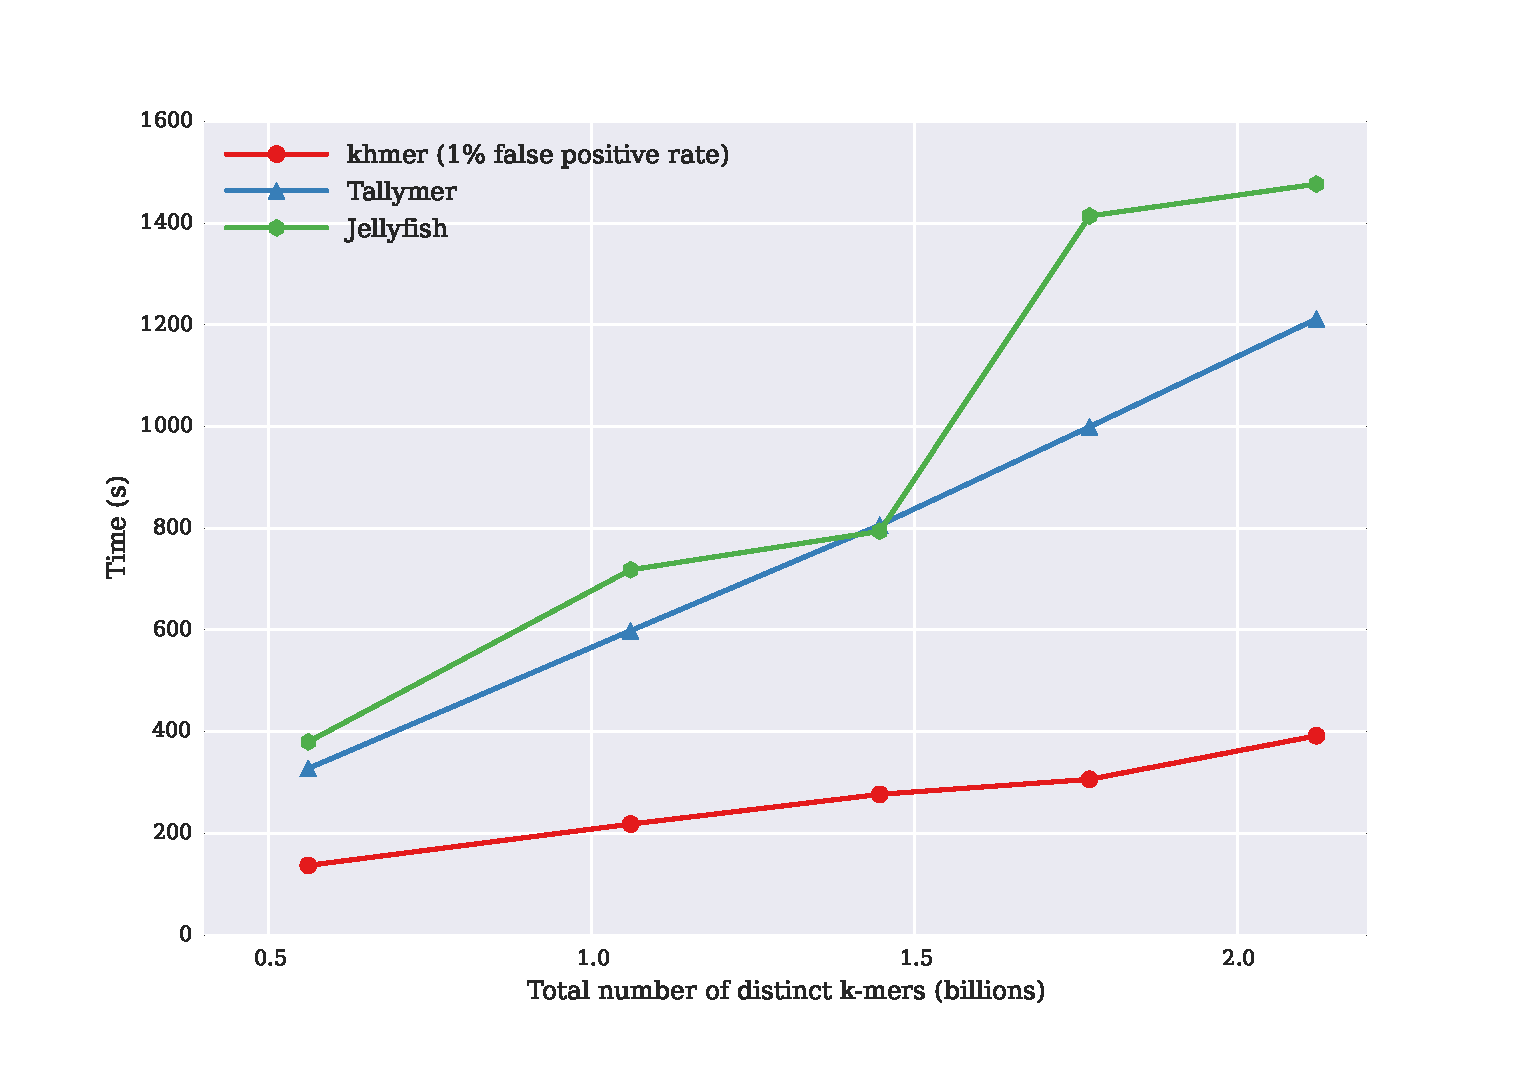
\includegraphics[width=5in]{./figures/figure4_count_benchmark}}
\caption{\bf Time for several k-mer counting tools to retrieve the
  counts of 9.7m randomly chosen k-mers (y axis), plotted against the
  number of distinct k-mers in the data set being queried (x axis).
  BFCounter, DSK, Turtle, KAnalyze, and KMC do not support this functionality.}
\label{fig:cmp_count}
\end{figure}


This highly  memory- and time-efficient online counting is particularly 
important for the streaming approaches to data
analysis needed as data set sizes increase, like digital normalization which 
will be discussed in next chapter and the IGS based method to analyze 
microbial diversity which will be discussed in later chapters.  Because query and
updating of k-mer counts can be done directly as data is being loaded,
with no need for disk access or an indexing step, khmer can also
perform well in situations with poor disk I/O performance.  (Note that
BFCounter also supports online k-mer counting \cite{Melsted2011}.)



\section{False positive rates in k-mer counting are low and predictable}

The Count-Min Sketch is a probabilistic data structure with a one-sided
error that results in random overestimates of k-mer frequency, but
does not generate underestimates. Next we will discuss the characteristics of 
such counting inaccuracy and the influence of such inaccuracy to the real-world 
applications of khmer for k-mer counting.

\subsection{The measured counting error is low on short-read data}


Due to the use of Count-Min Sketch and its lack of collision tracking,
khmer will report some incorrect counts for k-mers; these counts are
always higher than the true counts, up to the bound of 255 (a limit
imposed by our use of 8-bit counters).

In the Count-Min Sketch, the total memory usage is fixed; the memory
usage, the hash functions, and the total number of distinct objects
counted all influence the accuracy of the count.  While the
probability of an inaccurate count can easily be estimated based on
the hash table load, the miscount size is dependent on details of the
frequency distribution of k-mers \cite{Cormode2005}.

More specifically, in the analysis of the Count-Min Sketch, the
difference between the incorrect count and actual count is related to
the total number of k-mers in a data set and the size of each hash
table \cite{Cormode2005}. Further study has shown that the behavior of
Count-Min Sketch depends on specific characteristics of the data set
under consideration, like the distribution of k-mer abundances \cite{Rusu2008,
  CormodeM05}. In general, the average miscount will be small if the data is
left-skewed.  As noted by Melsted and Pritchard, a large number of
k-mers in short-read data are low-abundance, leading to precisely the
skew that would yield low miscounts \cite{Melsted2011}.  Here we use
both real and simulated data sets (Table \ref{table:random_data}) to evaluate the counting performance
in practice.

\begin{table}[!ht]
\caption{
\bf{Data sets used for analyzing miscounts.}}
\begin{tabular}{ | p{5cm} | c | c | c |}
\hline
Data set & Size of data set file & Number of total k-mers & Number of distinct k-mers \\
\hline
Real metagenomics reads                                  & 7.01M  & 2,917,200  & 1,944,996 \\
\hline
Totally random reads with randomly generated k-mers      & 3.53M  & 2,250,006  & 1,973,059 \\
\hline
Simulated reads from simulated genome with error         & 5.92M  & 3,757,479  & 2,133,592 \\
\hline
Simulated reads from simulated genome without error      & 9.07M  & 5,714,973  & 1,989,644 \\
\hline
Real {\em E. coli} reads                                        & 4.85M  & 4,004,911  & 2,079,302 \\
\end{tabular}
\begin{flushleft}
\end{flushleft}
\label{table:random_data}
\end{table}



\begin{figure}[!ht]
\centerline{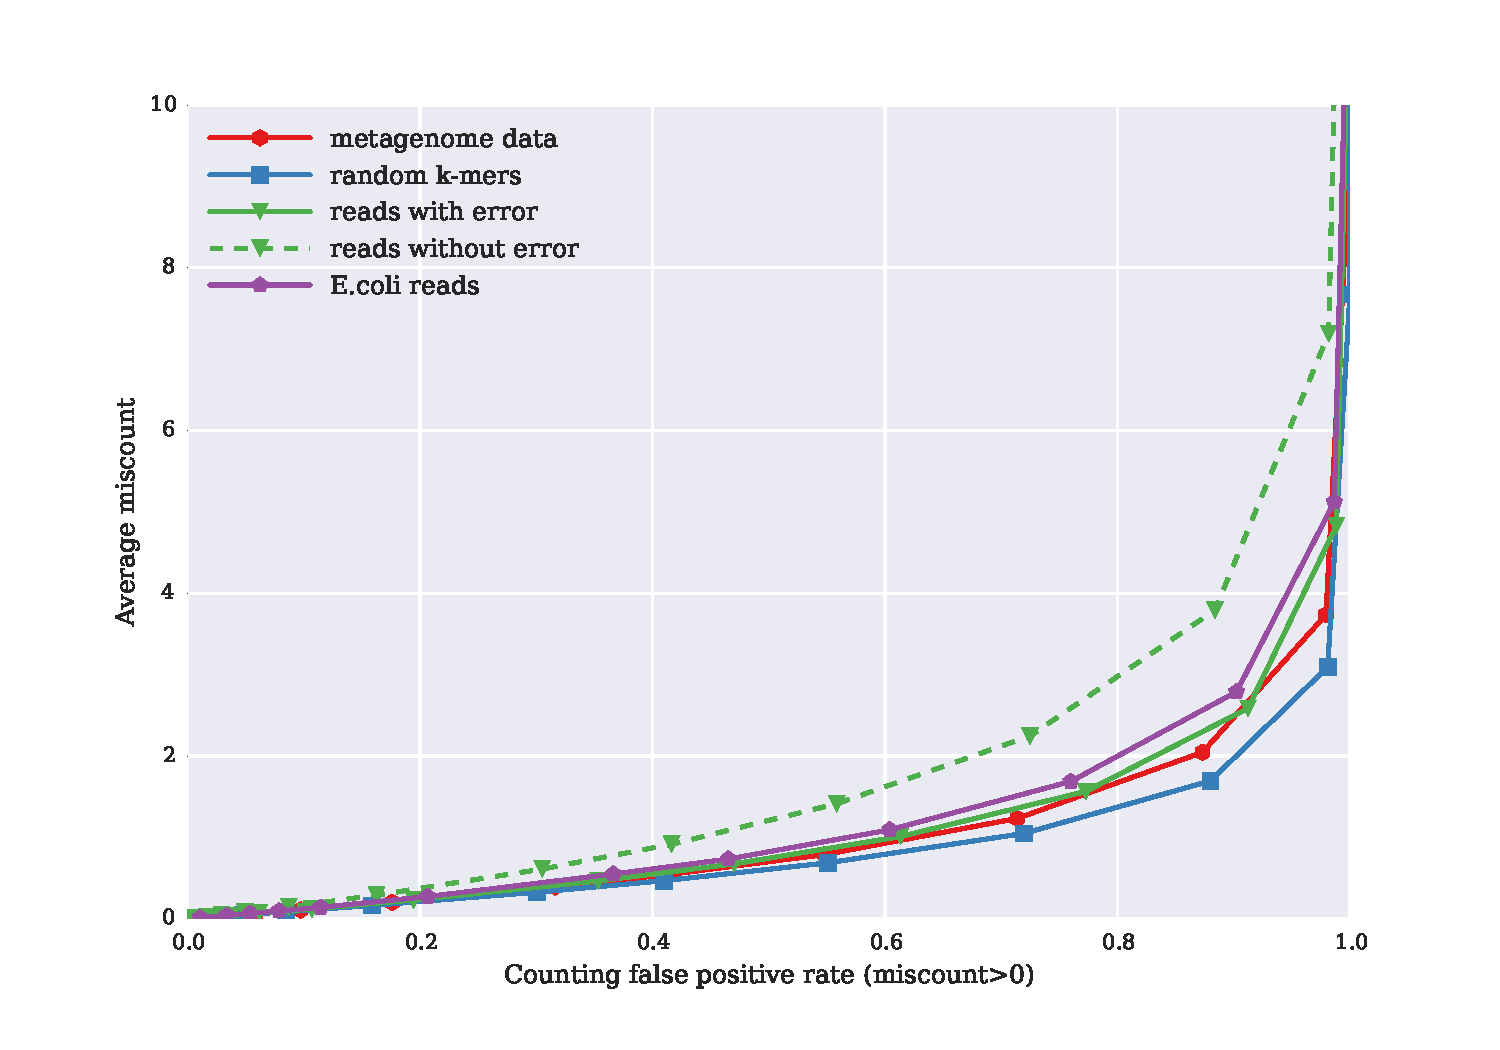
\includegraphics[width=5in]{./figures/figure5_average_offset_vs_fpr}}
\caption{\bf Relation between average miscount --- amount by which
the count for k-mers is incorrect --- on the y axis, plotted against
false positive rate (x axis), for five data sets.  The five data
sets were chosen to have the same total number of distinct k-mers: one
metagenome data set; a set of randomly generated k-mers; a set
of reads, chosen with 3x coverage and 1\% error, from a randomly generated
genome; a simulated set of error-free reads (3x) chosen from a randomly
generated genome and a set of {\em E. coli} reads.}
\label{fig:average_offset_vs_fpr}
\end{figure}

\begin{figure}[!ht]
\centerline{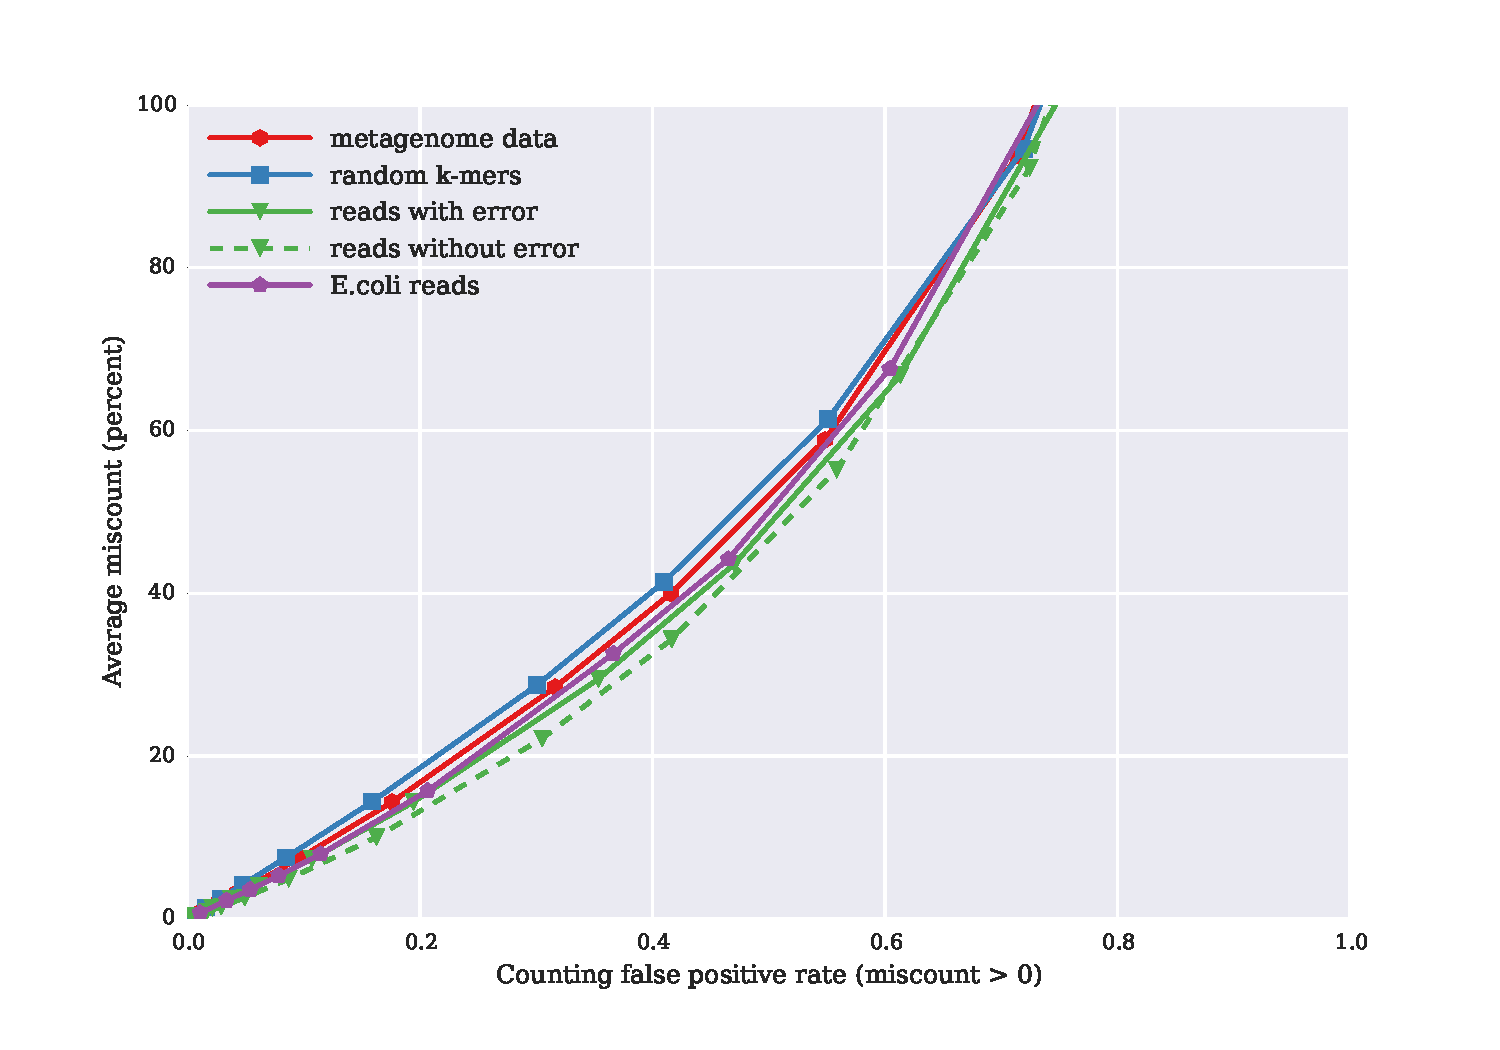
\includegraphics[width=5in]{./figures/figure6_percent_offset_vs_fpr}}
\caption{\bf Relation between percent miscount --- amount by which the
  count for k-mers is incorrect relative to its true count --- on the
  y axis, plotted against false positive rate (x axis), for five data
  sets.  The five data sets are the same as in Figure
  \ref{fig:average_offset_vs_fpr}.}
\label{fig:percent_offset_vs_fpr}
\end{figure}


Figure \ref{fig:average_offset_vs_fpr} shows the relationship between
average miscount and counting false positive rate for five different test data
sets with similar numbers of distinct k-mers: one metagenome data set;
a simulated set of random k-mers; a simulated set of reads, chosen
with 3x coverage and 1\% error; a simulated set of reads (3x) with no
error; and a set of {\em E. coli} reads (Table
\ref{table:random_data}).  Even when the counting false positive rate is as
high as 0.9 --- where 90\% of k-mers have an incorrect count --- the
average miscount is still below 4.

We separately analyzed the average {\em percentage} miscount between
true and false k-mers; e.g. an miscount of 4 for a k-mer whose true
count is 1 would be 400\%.  Figure \ref{fig:percent_offset_vs_fpr}
shows the relationship between average miscount and counting false
positive rate for the same five data sets as in Figure
\ref{fig:average_offset_vs_fpr}.  For a false positive rate of 0.1 (10\% of
k-mer counts are incorrect), the average percentage miscount is less
than 10\% for all five data sets; this will of course generally be
true, because the average miscount is bounded by the product of the
false positive rate with k-mer abundance.

We see here that for a fixed false positive rate, the simulated reads
without error have the highest average miscount, and the randomly
generated k-mers have the lowest average miscount.  This is because
these two abundance distributions have the least and most left-skew,
respectively: the simulated reads without error have no abundance-1
k-mers, while the randomly generated k-mers are entirely low
abundance. Thus, this counting approach is especially suitable for
high diversity data sets, such as metagenomic data, in which a larger
proportion of k-mers are low abundance or unique due to sequencing
errors.


For many applications, an approximate k-mer count is sufficient.  For
example, when eliminating reads with low abundance k-mers, we can
tolerate a certain number of low-frequency k-mers remaining in the
resulting data set falsely.  If RAM-limited we can do the filtering
iteratively so that at each step we are making more effective use of
the available memory.

In practice, we have found that a false positive rate of between 1\%
and 10\% offers acceptable miscount performance for a wide range of
tasks, including error profiling, digital normalization and
low-abundance read-trimming.  Somewhat surprisingly, false positive rates of up
to 80\% can still be used for both read trimming and digital
normalization in memory-limited circumstances, although multiple
passes across the data may be needed.

For many applications, the fact that khmer does not break an imposed
memory bound is extremely useful, since for many data sets ---
especially metagenomic data sets --- high memory demands constrain
analysis \cite{Howe2012,Luo2009}.  Moreover, because the false
positive rate is straightforward to measure, the user can be warned
that the results should be invalidated when too little memory is used.
When combined with the graceful degradation of performance for both
error trimming and digital normalization, khmer readily enables
analysis of extremely large and diverse data sets \cite{adina2013}. In
an experiment to assemble the reads of a soil metagenomic sample
collected from Iowa prairie, the number of reads to assemble drops
from 3.3 million to 2.2 million and the size of the data set drops from
245GB to 145GB accordingly after digital normalization
\cite{Howe2012}.  240GB memory was used in the process. This also
shows that khmer works well to analyze large, real-world metagenomic data
sets.


\subsection{Real-world applications for khmer}

Khmer has been widely used by many research groups for solving different 
bioinformatics problems. It is the foundation of all the work that
will be discussed in this thesis later. We will show the real-worl 
applications of khmer extensively in the chapters next. 

For many applications, an approximate k-mer count is sufficient.  For
example, when eliminating reads with low abundance k-mers, we can
tolerate a certain number of low-frequency k-mers remaining in the
resulting data set falsely.  If RAM-limited we can do the filtering
iteratively so that at each step we are making more effective use of
the available memory.

In practice, we have found that a false positive rate of between 1\%
and 10\% offers acceptable miscount performance for a wide range of
tasks, including error profiling, digital normalization and
low-abundance read-trimming.  Somewhat surprisingly, false positive rates of up
to 80\% can still be used for both read trimming and digital
normalization in memory-limited circumstances, although multiple
passes across the data may be needed.

For many applications, the fact that khmer does not break an imposed
memory bound is extremely useful, since for many data sets ---
especially metagenomic data sets --- high memory demands constrain
analysis \cite{Howe2012,Luo2009}.  Moreover, because the false
positive rate is straightforward to measure, the user can be warned
that the results should be invalidated when too little memory is used.
When combined with the graceful degradation of performance for both
error trimming and digital normalization, khmer readily enables
analysis of extremely large and diverse data sets \cite{adina2013}. In
an experiment to assemble the reads of a soil metagenomic sample
collected from Iowa prairie, the number of reads to assemble drops
from 3.3 million to 2.2 million and the size of the data set drops from
245GB to 145GB accordingly after digital normalization
\cite{Howe2012}.  240GB memory was used in the process. This also
shows that khmer works well to analyze large, real-world metagenomic data
sets.


% E.coli reads dataset has lower "coverage" than simulated reads without error.



\section{Conclusion}

K-mer counting is widely used in bioinformatics, and as sequencing
data set sizes increase, graceful degradation of data structures in
the face of large amounts of data has become important.  This is
especially true when the theoretical and practical effects of the
degradation can be predicted (see e.g. \cite{Melsted2011, Pell2012,
  Roy2014}).  This is a key property of the Count-Min Sketch approach,
and its implementation in khmer.

The khmer software implementation offers good performance, a robust
and well-tested Python API, and a number of useful and well-documented
scripts.  While Jellyfish, DSK, KMC, and Turtle also offer good
performance, khmer is competitive, and, because it provides a Python
API for online counting, is flexible.  In memory-limited situations
with poor I/O performance, khmer is particularly useful, because it
will not break an imposed memory bound and does not require disk
access to store or retrieve k-mer counts.  However, in exchange for
this memory guarantee, counting becomes increasingly incorrect as less
memory is used or as the data set size grows large; in many situations
this may be an acceptable tradeoff.

\section{Data}

\subsection{Code and data set availability}

% @CTB update

The khmer software \cite{khmer} is implemented in C++ in a Python
wrapper, enabling flexible use and reuse by users with a wide range of
computational expertise.  The software package is freely available for
academic and commercial use and redistribution under the BSD license
at github.com/ged-lab/khmer/.  khmer comes with substantial
documentation and many tutorials, and contains extensive unit tests.
Moreover, we have built several applications on top of khmer,
including memory-efficient de Bruijn graph partitioning
\cite{Pell2012} and lossy compression of short-read data sets for
assembly \cite{Brown2012}.

The version of khmer used to generate the results in this chapter is available
at \\
http://github.com/ged-lab/khmer.git, tag '2013-khmer-counting'.
Scripts specific to this paper are available in the paper repository
at \\
https://github.com/ged-lab/2013-khmer-counting.
The IPython\cite{4160251} notebook file and data analysis to generate the figures are also
available in that github repository.  Complete instructions to reproduce
all of the results in this paper are available in the khmer-counting
repository; see README.rst.

\subsection{Sequence Data}

One human gut metagenome reads data set (MH0001) from the 
MetaHIT (Metagenomics of the Human Intestinal Tract) project \cite{Qin2010} was used. 
It contains approximately 59 million reads, each 44bp long; it was trimmed to remove 
low quality sequences. 

Five soil metagenomics reads data sets with different size were taken
from the GPGC project for benchmark purpose (see Table
\ref{table:datasets}).  These reads are from soil in Iowa region and they
are filtered to make sure there are less than 30\% Ns in the read and
each read is longer than 30 bp.  The exact data sets used for the
paper are available on Amazon S3 and the instructions to acquire these
data sets are available in the paper repository on github.com.

We also generated four short-read data sets to assess the false
positive rate and miscount distribution. One is a subset of a real
metagenomics data set from the MH0001 data set, above. The second
consists of randomly generated reads. The third and fourth contain
reads simulated from a random, 1 Mbp long genome.  The third has a
substitution error rate of 3\%, and the fourth contains no errors. The
four data sets were chosen to contain identical numbers of distinct
22-mers.  The scripts necessary to regenerate these data are available
in the paper repository on github.com.



